\section{Online evaluation}
\begin{figure}[ht]
	\centering
	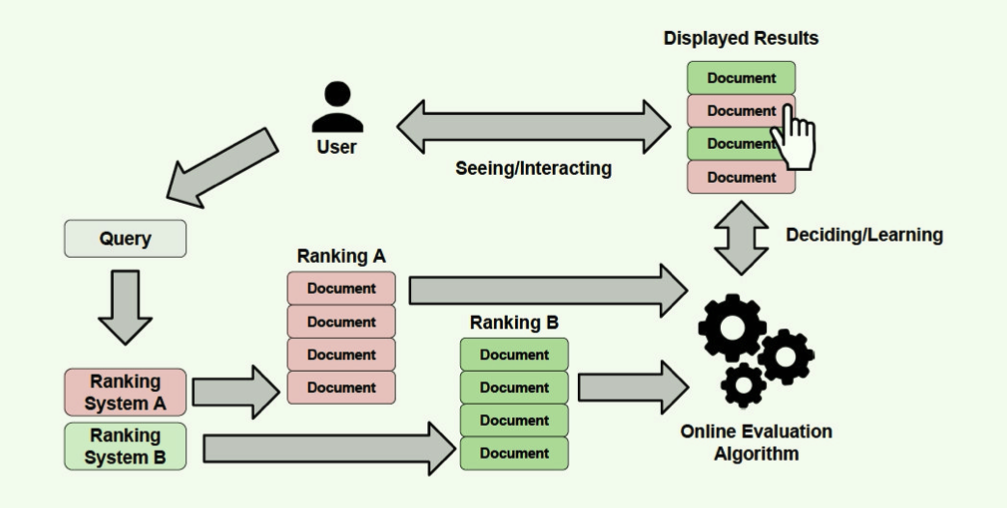
\includegraphics[width=0.6\textwidth]{figures/online_evaluation.png}
	\caption{Schema of Online Evaluation}
	\label{img:online_eval}
\end{figure}
\begin{itemize}
	\item In online evaluation, the system interacts with the user $\implies$ user "tells" what is relevant (through interactions), system analyzes the user's behavior for gaining knowledge about preferences/relevances
	\item The benefit of online evaluations is that they are mostly simpler and more efficient (as they have control over what data is collected) and directly incorporate measuring the ranking quality
	\item online evaluation systems have control over what to display to user
	\item However, the downsides are that the results are worse to explain/interpret (why did users click less, different queries might rely on different metrics, ...). Also, evaluations might not be comparable over time so that we also need to ensure the same conditions/user population for both systems.
	\item An schematic figure is given in Fig. \ref{img:online_eval}
	\item An online evaluation algorithm should
	\begin{itemize}
		\item give reliable and correct results (robust to noise, handle biases)
		\item provide good user experience
	\end{itemize} 
\end{itemize}
\subsection{Analyzing user behavior}
\begin{itemize}
	\item A user provides various signals from which we can try to retrieve his "happiness" about the results. The following ones are mostly used:
	\item \textit{Clicks} - clicks are mostly noisy so that a click doesn't ensure that the document was actually relevant. Clicks have several biases:
	\begin{itemize}
		\item \textit{Position bias} - a user tends towards clicking higher ranked results
		\item \textit{Contextual bias} - nearby results effect the click probability of a document
		\item \textit{Attention bias} - some results draw more attention to themselves by the usage of images, font size, ...
	\end{itemize}
	\item \textbf{Time} - the time a user spends on a certain query before coming back to search engine
	\begin{itemize}
		\item \textit{Dwell time} - time spent on a clicked page. If duration is more than 30 seconds, we assume that click satisfied
		\item \textit{Exit type} - how the user exists the page (closing browser, continue scrolling through results, putting in new query, ...) 
	\end{itemize}
	\item \textit{Mouse movement} - time on website is not sufficient. Mouse movement can indicate whether user is actually reading or only scrolling/scanning
	\item \textit{Reformulations} - if new query is entered, check for similarity with the previous one. Reformulated/Similar queries that were entered quickly after the first one, indicate that user was not satisfied with previous results.
\end{itemize}
\subsection{A/B Testing}
\begin{itemize}
	\item When testing two systems in an online experiment, we need to make sure that both have the same preconditions so that the system improvements clearly correlate with the new click/sale numbers
	\item In A/B Testing, users are split into two groups where each group is assigned to one of the algorithms. We analyze the users' behavior on both systems and calculate a metric based on that. Comparing the results for both systems on significance leads to a final decision.
	\item \textbf{Advantages}
	\begin{itemize}
		\item straightforward and common
		\item can test many different aspects
	\end{itemize}
	\item \textit{Challenges} in A/B Testing
	\begin{itemize}
		\item If one system is very different and probably bad, it will affect the \textit{user experience} and damages website image $\implies$ perform offline evaluation in advance to avoid testing a very bad system
		\item It is hard to define \textit{metrics} as they can contradict each other. For example, if we report number of clicks and sessions per users, a click increase can indicate better/more relevant results. However, if another systems provides snippets that already contain the information, the user will click less.
		\item The metric should be as sensitive as possible. \textit{Sensitivity} is the ability of the metric to detect the statistically significant difference when the treatment effect exists $\implies$ how many queries/days/users/... for significance needed?
		\item they are inefficient and require lots of data
		\item tests have to run for a long time
		\item need to identify individual users
	\end{itemize}

	\begin{figure}[ht]
		\centering
		\includegraphics[width=0.5\textwidth]{figures/online_eval_AB_testing.png}
		\caption{Visualization of A/B Testing}
		\label{img:online_eval_AB_testing}
	\end{figure}
\end{itemize}
\subsection{Interleaving}
\begin{itemize}
	\item A/B testing introduces a high variance by letting different users evaluate different systems $\implies$ Show interleaved results from both algorithms A and B without telling the user which document is from which model
	\item The evaluation is based on the clicks of a user where the algorithm gets the credit that provided the clicked document
\end{itemize}
\subsubsection{Balanced interleaving}
\begin{itemize}
	\item In balanced interleaving, we select randomly which algorithm starts (A or B). If A would start, we take the first document of A and place it in our interleaved ranking list. Then we pick the first document of B and continue with A again
	\item If a document is already in the interleaved ranking, we skip this document and continue with picking the next document from the \textit{other} ranking model 
	\begin{figure}[ht]
		\centering
		\includegraphics[width=0.5\textwidth]{figures/online_eval_balanced_interleaving.png}
		\caption{Formal algorithm describing balanced interleaving}
		\label{img:online_eval_balanced_interleaving}
	\end{figure}
	\item Problem: balanced interleaving brakes under corner cases. Assume following ranking:
	$$A: \left\{d_1, d_2, d_3, d_4\right\}, B: \left\{d_2, d_3, d_4, d_1\right\}$$
	No matter whether we start at model A or B, the interleaved list contains three documents assigned to B and only one to A. Thus, random clicking would lead to B winning $\implies$ bias. Resolved by team-draft interleaving
\end{itemize}
\subsubsection{Team-draft interleaving}
\begin{itemize}
	\item In team-draft interleaving we guarantee that both algorithms contribute equally to the interleaved ranking
	\item Process:
	\begin{enumerate}
		\item Until $k$ documents are placed:
		\begin{enumerate}
			\item randomly choose ranker A or B
			\item let chosen ranker place its next unplaced document
			\item let other ranker place its next unplaced document
			\item remember which ranker placed which document
		\end{enumerate}
		\item present interleaving to user, observe clicks
		\item ranker with most clicks on its placed documents wins
	\end{enumerate}
	\item Team-draft interleaving finds no preference under random clicks (e.g. 50\% chance that second document is clicked $\rightarrow$ equal for both A and B as they are equally likely to place second document)
	\item Properties of team-draft interleaving: 
	\begin{itemize}
		\item more efficient than A/B testing (needs less samples)
		\item user experience hardly effectly (not worse than worst ranker)
		\item correctness: ranker that placed clicked documents higher \textit{usually} wins
	\end{itemize}
	\item Problematic case for team-draft interleaving (document 3 being the only relevant document) in Fig. \ref{img:team_draft_interleaving_problem}
	\begin{figure}[h!]
		\centering
		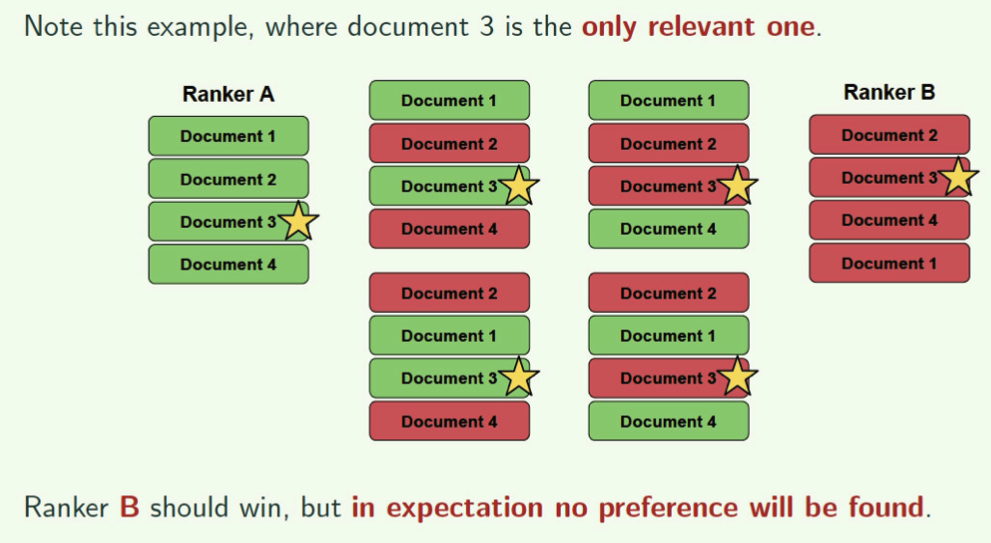
\includegraphics[width=0.6\textwidth]{figures/team_draft_interleaving_problem.png}
		\caption{Edge Case of Team-Draft Interleaving}
		\label{img:team_draft_interleaving_problem}
	\end{figure}
\end{itemize}
\subsubsection{Probabilistic interleaving}
\begin{itemize}
	\item To avoid biases completely, we can apply probabilistic models
	\item Convert the ranking of each model to a probability distribution by applying softmax ($\tau \in \mathbb{R}^+$) for ranker $R_A$:
	$$P(d|D,R_A) = \frac{\frac{1}{rank(d,R_A)^{\tau}}}{\sum_{d' \in D} \frac{1}{rank(d',R_A)^{\tau}}}$$
	\item Process:
	\begin{enumerate}
		\item compute $P_A$ and $P_B$ from ranker A and B
		\item repeat until $k$ documents placed:
		\begin{enumerate}
			\item randomly choose $P_A$ or $P_B$ and sample document $d$
			\item place $d$ and remember which ranker placed it
			\item renormalize $P_A$ \textit{and} $P_B$ after removing $d$
		\end{enumerate}
		\item display to user and observe clicks
		\item ranker with the most clicked documents wins
	\end{enumerate}
	\item We expect the same number of clicks for documents at the same position of both algorithms due to the same probability in the softmax.
	\item Does this method have fidelity?
	\begin{itemize}
		\item no ranker has advantage due to factors other than relevance as every ranker is equally likely to place at every rank
		\item unambiguous winner will always win in expectation as every ranker is equally likely to place at every rank $\rightarrow$ dominating ranker is more likely to place relevant documents at each rank $\rightarrow$ if relevant documents are more likely to be clicked, dominating ranker wins in expectation
	\end{itemize}
\end{itemize}
\textbf{Probabilistic Interleaving with expected outcome}
\begin{itemize}
	\item Another, more efficient evaluation method is by marginalizing over all possible assignments. instead of using the outcome based on the ranker assignments, we calculate expected outcome over all possible ranker assignments
	\item let outcome of comparison be $O(R_A,R_B,L,T,c) \in \{-1,0,1\}$ where $L$ is the interleaved list, assignments $T$, clicks $c$
	\item since clicks are independent of assignment $T$, we can marginalize:
	$$ \mathbb{E}[O(R_A,R_B,L,c)] = \sum_T P(T|R_A,R_B,L)O(R_A,R_B,L,T,c)$$
	\item the placement probability is therefore:
	\begin{align*}
		&P(T_i=A) = 0.5 \\
		&P(L_i = d|T_i = A) = P_A(d) = \dfrac{\dfrac{1}{rank(d,R_A)^\tau}}{\sum_{d' \in D} \dfrac{1}{rank(d',R_A)^\tau}} \\
		&P(T_i = A|L_i=d) = \dfrac{P_A(d)}{P_A(d) + P_B(d)}
	\end{align*}
	\item using that the outcome of a comparison is only dependent on the clicked documents and the assignment of a document does not depend on other assignments, we only have to consider the possible assignments of the \textit{clicked} documents (bringing complexity from $2^k$ to $2^c$)
	\item Process:
	\begin{enumerate}
		\item compute $P_A$ and $P_B$ from ranker A and B
		\item repeat until $k$ documents placed:
		\begin{enumerate}
			\item randomly choose $P_A$ or $P_B$ and sample document $d$
			\item place $d$ without remembering which ranker placed it
			\item renormalize $P_A$ \textit{and} $P_B$ after removing $d$
		\end{enumerate}
		\item display to user and observe clicks
		\item calculate expected outcome by marginalizing over all possible placements
		\item expected winner wins competition
	\end{enumerate} 
	\item Note that compared to a hard assignment of 0 or 1 in balanced and team draft interleaving, the credit accumulated for clicks is smoothed based on the relative rank of the document in the original result lists (a click on any document leads to a non-zero credit for both rankings)
	\item Figure~\ref{img:online_eval_probabilistic_interleaving_2} visualizes an example for probabilistic interleaving
	\begin{figure}[ht]
		\centering
		\includegraphics[width=\textwidth]{figures/online_eval_probabilistic_interleaving_2.png}
		\caption{Visualization of probabilistic interleaving}
		\label{img:online_eval_probabilistic_interleaving_2}
	\end{figure}
\end{itemize}
\textbf{Properties of probabilistic interleaving}
\begin{itemize}
	\item correctness: 
	\begin{itemize}
		\item correct outcomes guaranteed w.r.t. fidelity
		\item marginalization does not affect expected outcomes
	\end{itemize}
	\item User experience:
	\begin{itemize}
		\item not guaranteed
		\item every possible ranking can be displayed, albeit with different probabilities
	\end{itemize}
\end{itemize}
\subsubsection{Optimized interleaving}
\begin{itemize}
	\item look at allowed interleavings: produce rankings by always looking at the top documents, not yet placed $\rightarrow$ never have a document, where both rankers agree that another document should come first
	\item can use different scoring functions (there are requirements). A click on a document gives a preference score determined how document is ranked:
	\begin{itemize}
		\item Linear Rank Difference:
		$$s(d,R_A,R_B) = \delta_d = rank(d,R_A) - rank(d, R_B)$$
		\item Inverse Rank Difference:
		$$s(d,R_A,R_B) = \delta_d = \dfrac{1}{rank(d,R_A)} - \dfrac{1}{rank(d, R_B)}$$
	\end{itemize}
	\item This gives us Fig \ref{img:optimized_interleaving}
	\begin{figure}[h!]
		\centering
		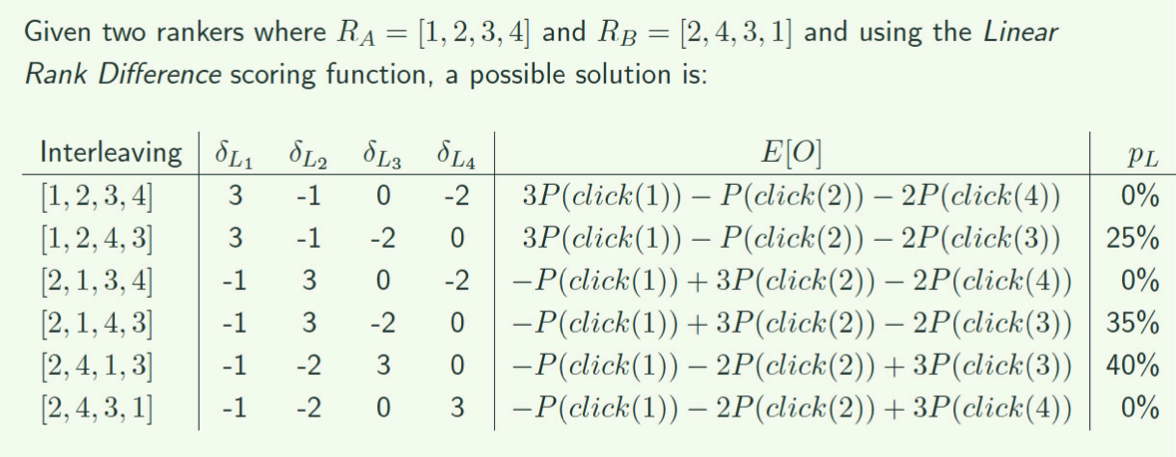
\includegraphics[width=\textwidth]{figures/optimized_interleaving.png}
		\caption{Optimized Interleaving}
		\label{img:optimized_interleaving}
	\end{figure}
	where, if the probability $p_L$ of interleaving $L$ being displayed, the expected outcome can be written as:
	$$\mathbb{E}[O] = \sum_{L \in \mathcal{L}} \Big( p_L \sum_{i=1}^{|L|} P(click(i))s(L_i,R_A,R_B) \Big) = 0$$
	which becomes a linear optimization task to find $p_L$
	\item We used randomization to check that under randomized clicks there is no winner
	\item Properties of optimized interleaving:
	\begin{itemize}
		\item user experience: strongest guarantees of all interleaving methods
		\item correctness: method has fidelity (if optimized for it) as long as linear optimization is successful (it has been proven by brute force that there always is a solution for top-10 rankings)
		\item can be correct under other definitions as well
	\end{itemize}
\end{itemize}